
\subsection{Introduction to Digital Image Processing}
{\color{red} REMOVE section}
 
Digital images are represented as a two-dimensional function, f(x,y), where x and y are plane (spatial) coordinates each representing one pixel. Each pixel has a finite value that represents the intensity, colors, depth, gray levels etc. To represent a color, OpenCV use the BGR color space. That means that each pixel contains an array with 3 values, [Blue, Green, Red], where the values are normally an integer between 0 and 255. The BGR color space is shown in figure \ref{fig:bgr_color_space}.

\begin{figure}[h]
    \centering
    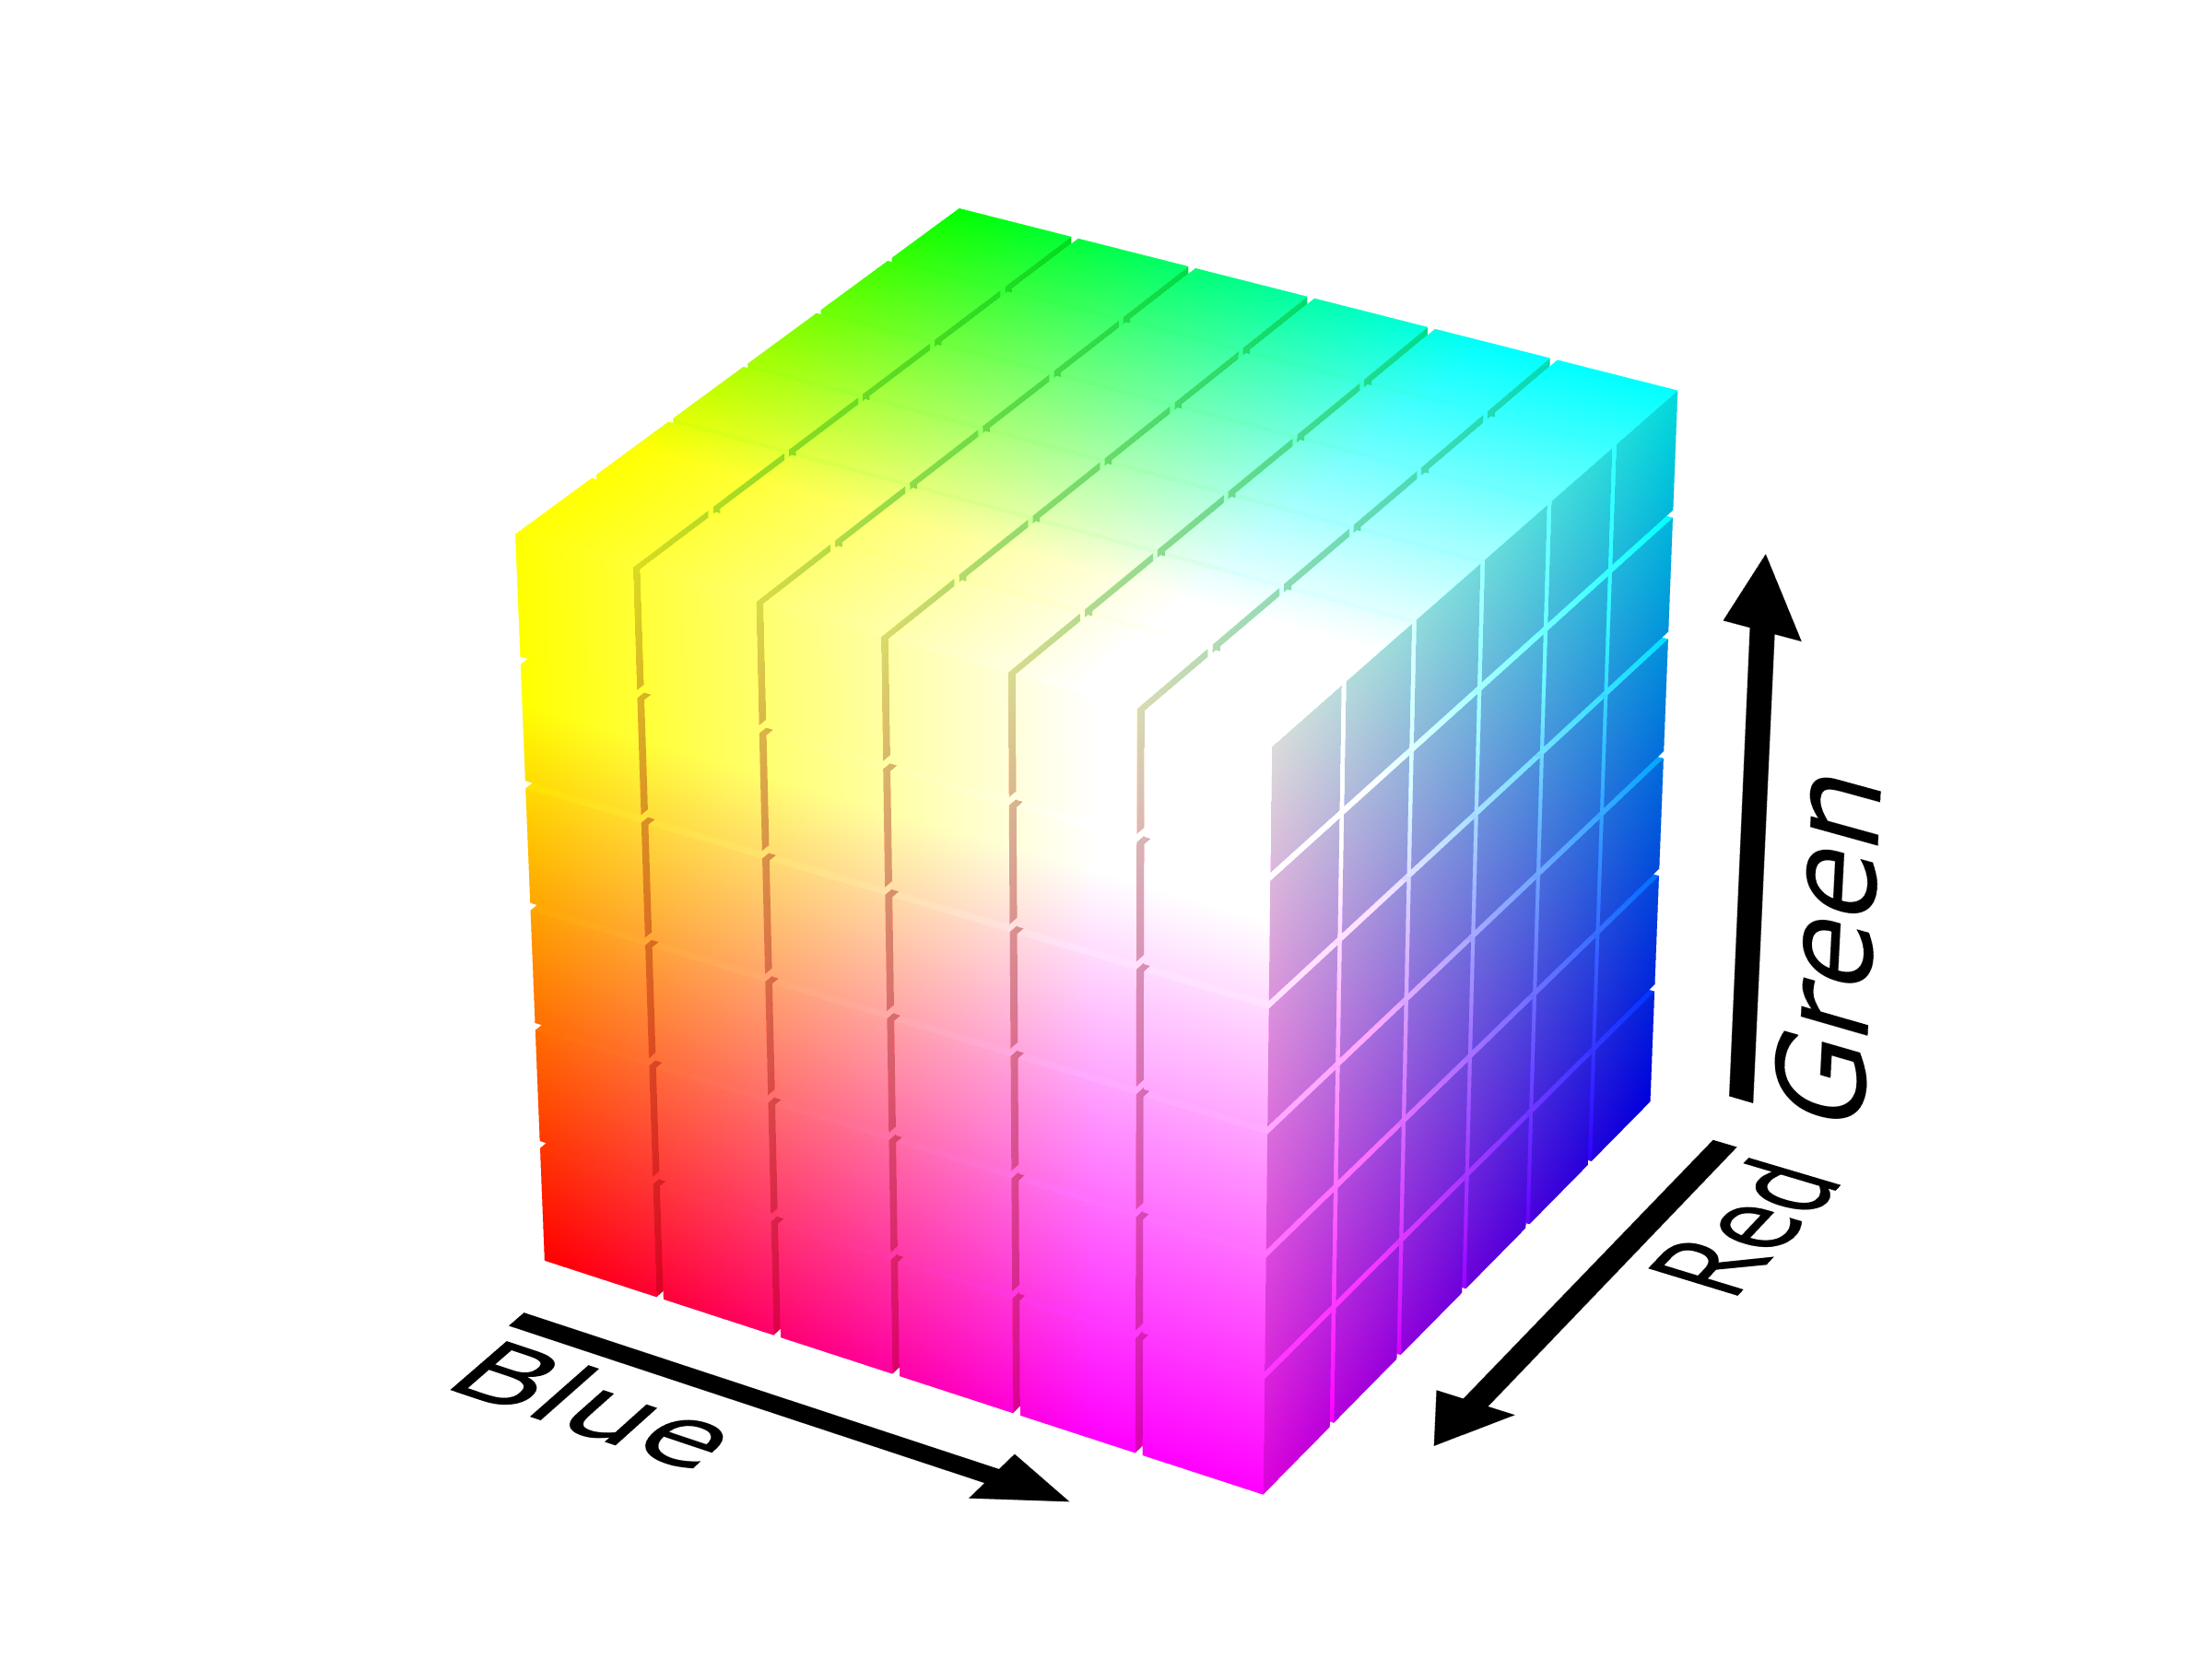
\includegraphics[width=.9\linewidth]{images/introduction/RGB_color_solid_cube}
    \caption{BGR color space}
    \label{fig:bgr_color_space}
\end{figure}

Digital image processing is the use of computer algorithms to perform some processing on a digital image. Through the use of image processing it is possible to achieve simple things as changing the color space, to more advanced things as object recognition and scene understanding. Digital image processing is used today for important tasks as medical visualisation and industrial inspection, but also just as filters on Instagram to make someone look tanner. 

Digital image processing has many areas of use, listed below are some of the most important ones:
\begin{itemize}
\item Visualization - observe objects that are not visible.
\item Classification - decide what kind of object is in the image.
\item Image sharpening or restoration - enhance the image quality.
\item Pattern recognition - used in machine learning to recognize patterns and regularities in the image data.
\item Projection - image of a three-dimensional object is projected into a planar surface. Used in technical drawing.
\item Linear filtering - filter out data from images.
\end{itemize}

\cite{book:digital_image_processing, book:machine_vision}

{\color{red}Add image examples???}






{\color{red}
Innledning: Create a research space (CARS)
• Presenter forskningsområdet («establish territory»)
    • Presenter tema og kunnskapsstatus i feltet
• Vis behov/nødvendigheten for din forskning («establish niche»)
    • Bygg på tidligere forskning
    • Vis at kunnskap er manglende/fraværende
    • Vis spørsmål/konflikter ved tidligere forskning
• Presenter din forskning («occupy niche»)
    • Hva vil du oppnå?
    • Uttrykt gjennom hypotese, formål eller forskningsspørsmål
    • På hvilken måte kan prosjektet ditt bidra til ny kunnskap?


Handler altså om: HVA og HVORFOR
Beskriv konteksten/feltet/bakgrunn – og motiver egen forskning (Hva og Hvorfor)

• Hva
    • Hva handler prosjektet ditt om (tema)?
    • Hva gjør du i prosjektet ditt?
    • Hva ønsker du å oppnå/finne ut?
• Hvorfor (motivasjon)
    • Hvorfor er det viktig å undersøke/skrive om det?
    • Har andre undersøkt problemet? Hva har de funnet?
    • Hva skal prosjektet ditt bidra til – hvilket «kunnskapshull» skal det fylles?


Undersøke innledningen
• Hvordan er innledningen delt inn? Hvilke underkapitler?
• Hva gjør skriveren i første avsnitt?
    • «Beveger» teksten seg «fra det generelle til det spesifikke» – og på hvilken måte?
• Ser du kildehenvisninger – hva brukes de til?


}




\subsection{Different Levels of Particle Noise}

To make the algorithm suitable for different conditions of water, noise was added to the depthmap.
The original plan was for the water to get blurry by it self since the dead salmons rotting process is very quick. The water, at the end of picture taking, looked very blurry and filled with particles, but it did not show much differences in the depthmap image. It's not known if it is mostly the water mediums properties that causes noise in the depthmap, and that particles are not enlarging this disorder significantly, or if enough particles within reason will disturb the depth measurements done by the Raytrix.

Since we could not get the naturally disturbances in the water to affect the depthmap directly, noise was added to the computed depthmap images.

The noise used is salt and pepper noise, which turns a random set of pixels into either black or white. For the noise to illustrate real particles in different size and shape, morphological closing was added to the salt and pepper noise before the mask was added to the depthmap image.


\subsubsection{Level 1}

Noise level 1 is the original images taken by the Raytrix camera, without extra noise added.
The result from these images can be seen in section \ref{section:depthmap}.


\subsubsection{Level 2}

Noise level 2 has some salt and pepper noise added to it. Figure \ref{fig:noise_level_2} shows the resulting depthmap and the result using the same approach as described in section \ref{section:depthmap}.

\begin{figure}[h]
    \centering
    \begin{subfigure}{\textwidth}
        \centering
        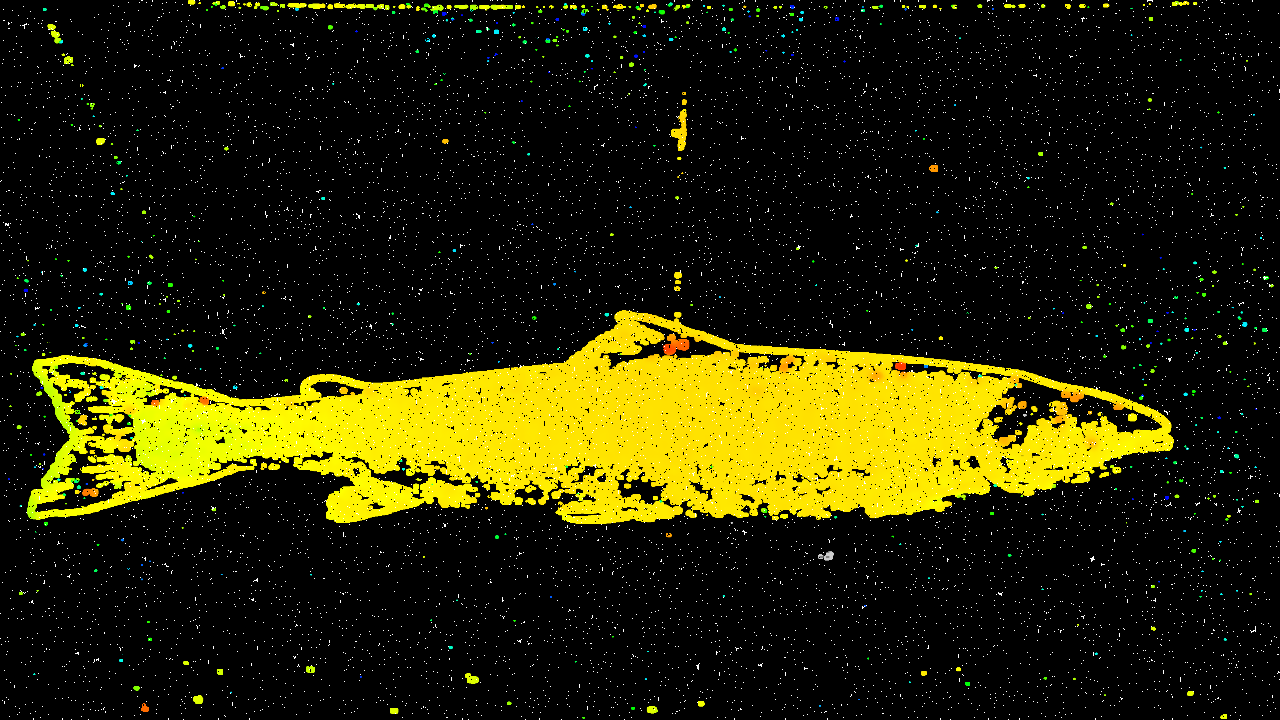
\includegraphics[width=.7\linewidth]{images/implementation/noise_level_2/1_original}
        \caption{Depthmap image with noise level 2} 
        \label{fig:noise_level_2_original}
    \end{subfigure}\hspace*{\fill}
    
    \medskip
    \begin{subfigure}{\textwidth}
        \centering
        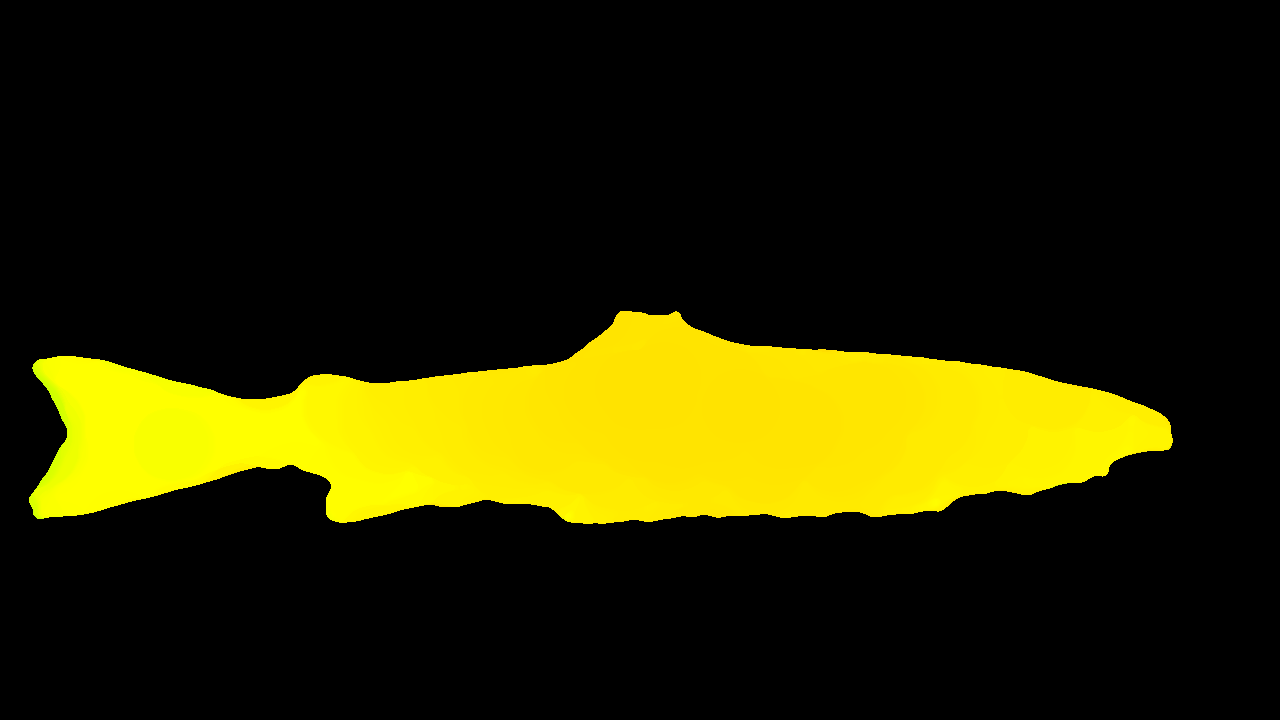
\includegraphics[width=.7\linewidth]{images/implementation/noise_level_2/7_median_filter}
        \caption{Resulting depthmap} 
        \label{fig:noise_level_2_result}
    \end{subfigure}\hspace*{\fill}
    \caption{Depthmap image and result for noise level 2}
    \label{fig:noise_level_2}
\end{figure}


\subsubsection{Level 3}

Noise level 3 has more salt and pepper noise that noise level 2, and the noise is morphologically closed more times. The noisy image and the result after using the algorithm from section \ref{section:depthmap} can be seen in figure \ref{fig:noise_level_3}.

\begin{figure}[h]
    \centering
    \begin{subfigure}{1\textwidth}
        \centering
        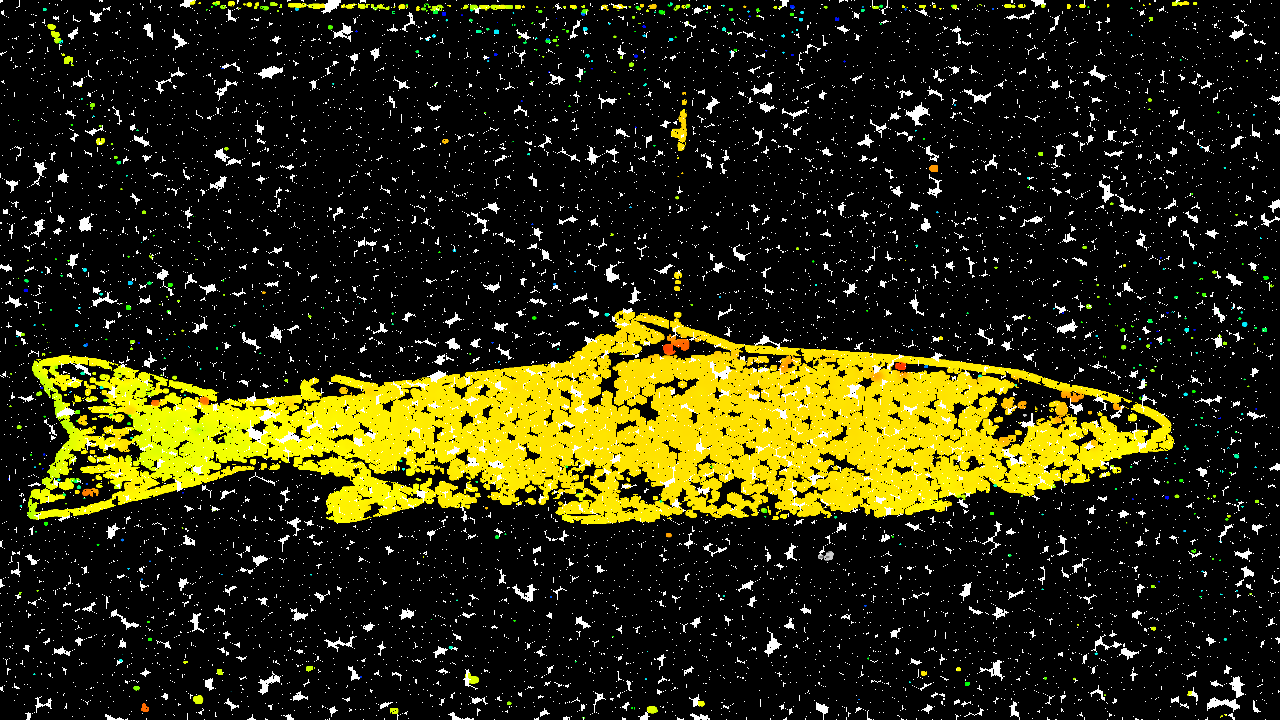
\includegraphics[width=.7\linewidth]{images/implementation/noise_level_3/1_original}
        \caption{Depthmap image with noise level 3} 
        \label{fig:noise_level_3_original}
    \end{subfigure}\hspace*{\fill}
    
    \medskip
    \begin{subfigure}{1\textwidth}
        \centering
        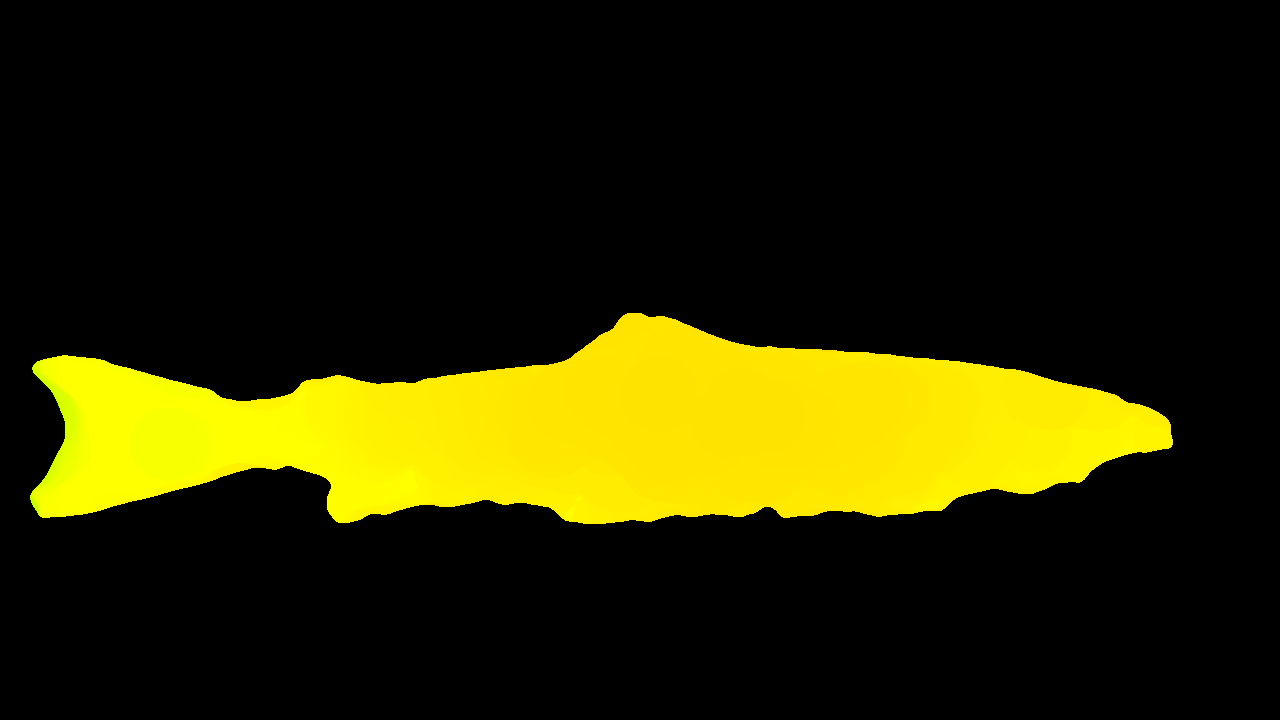
\includegraphics[width=.7\linewidth]{images/implementation/noise_level_3/7_median_filter}
        \caption{Resulting depthmap} 
        \label{fig:noise_level_3_result}
    \end{subfigure}\hspace*{\fill}
    \caption{Depthmap image and result for noise level 3}
    \label{fig:noise_level_3}
\end{figure}






\subsection{Motivation}

The work done in this report is done in cooperation with Sensomar AS (SEALAB OCEAN GROUP).
Sensomar SEALAB is a company developing camera systems for underwater use. Most of SEALABs technology is planned for use in the fishing industry, especially aimed towards salmon breeding industry. 

The aquaculture industry has grown dramatically over the last decades, and the fishing industry has become more and more industrial. This industrialisation of fish breeding has made the production more profitable, but it has also caused the concentration of salmon lice to grow dramatically. With the use of good camera systems along with the right image processing it can be possible to detect the lice much earlier than now. 

Another challenge for the fish breeding companies is estimation of biomass. A grown salmons weight can vary from around two to ten kilos. This makes it hard for the companies to know the volume of fish they have in their cages at any time, and difficult to know how much fish they can sell. If they sell more fish then the cage contains they need to purchase fish from competitors at a steep price. The biomass estimation directly effects the profit, therefore, providing a solution for biomass estimation would very much benefit the companies. 

SEALABs current goal is to develop an advanced underwater camera system that can both detect salmon lice and measure biomass in the fish cages.
The system currently used by SEALAB for the biomass estimation is the Raytrix R42 camera, a light field camera computing both 2D and 3D images with corresponding depth data in one frame. The camera is the best in its field. Features for the Raytrix R42 camera is explained is section \ref{the_raytrix_camera}. 
The depthmap produced by the cameras software can be used to estimate the volume of an object. Depthmaps computed by the Raytrix is very accurate in air, but underwater, the depthmap is not as accurate. Reasons for this inaccuracy can come directly from the water mediums properties, it can depend on the lightning, the background and/or particles in the water. This means that even though the best available camera technology is used, the results directly is still not good enough for correct volume measurement.

With the use of image processing for noise and particle removal, together with testing of different lightning and background conditions, it is reasonable to believe that the estimates for biomass of fish could be improved.

This report shows the exploration of different processing possibilities done on data extracted from the Raytrix R42. Different testing conditions is explored, and a suggested solution is provided and tested.




%%%%%%%%%%%%%%%%%%%%%%%%%%%%%%%%%%%%%%%%%%%%%%


This camera is therefore very useful for industrial purposes, as you can get both a clear image, a depthmap, and a 3D model of the scene.

 The Raytrix cameras has no documented usage underwater, and since the physical properties of water cause degradation effects not present in air, the depth measurements get affected.


%%%%%%%%%%%%%%%%%%%%%%%%%%%%%%%%%%%%%%%%%%%%%%


\subsection{Shadow Removal {\color{red}Remove?}}
There are few open source algorithms for shadow removal. There are some advanced explanations for shadow removal, but they do not always work properly. Shadow removal can be useful when reconstructing an image or when detecting objects. 
Simple shadow removal can be done by transforming the color space of the image from RBG to HSV and then setting the value component of each pixel to a constant value. What this really does is even out all grey tones in the image, as is shown in figure \ref{fig:shadow_removal}.

\begin{figure}[h]
    \centering
    \begin{subfigure}{0.5\textwidth}
        \centering
        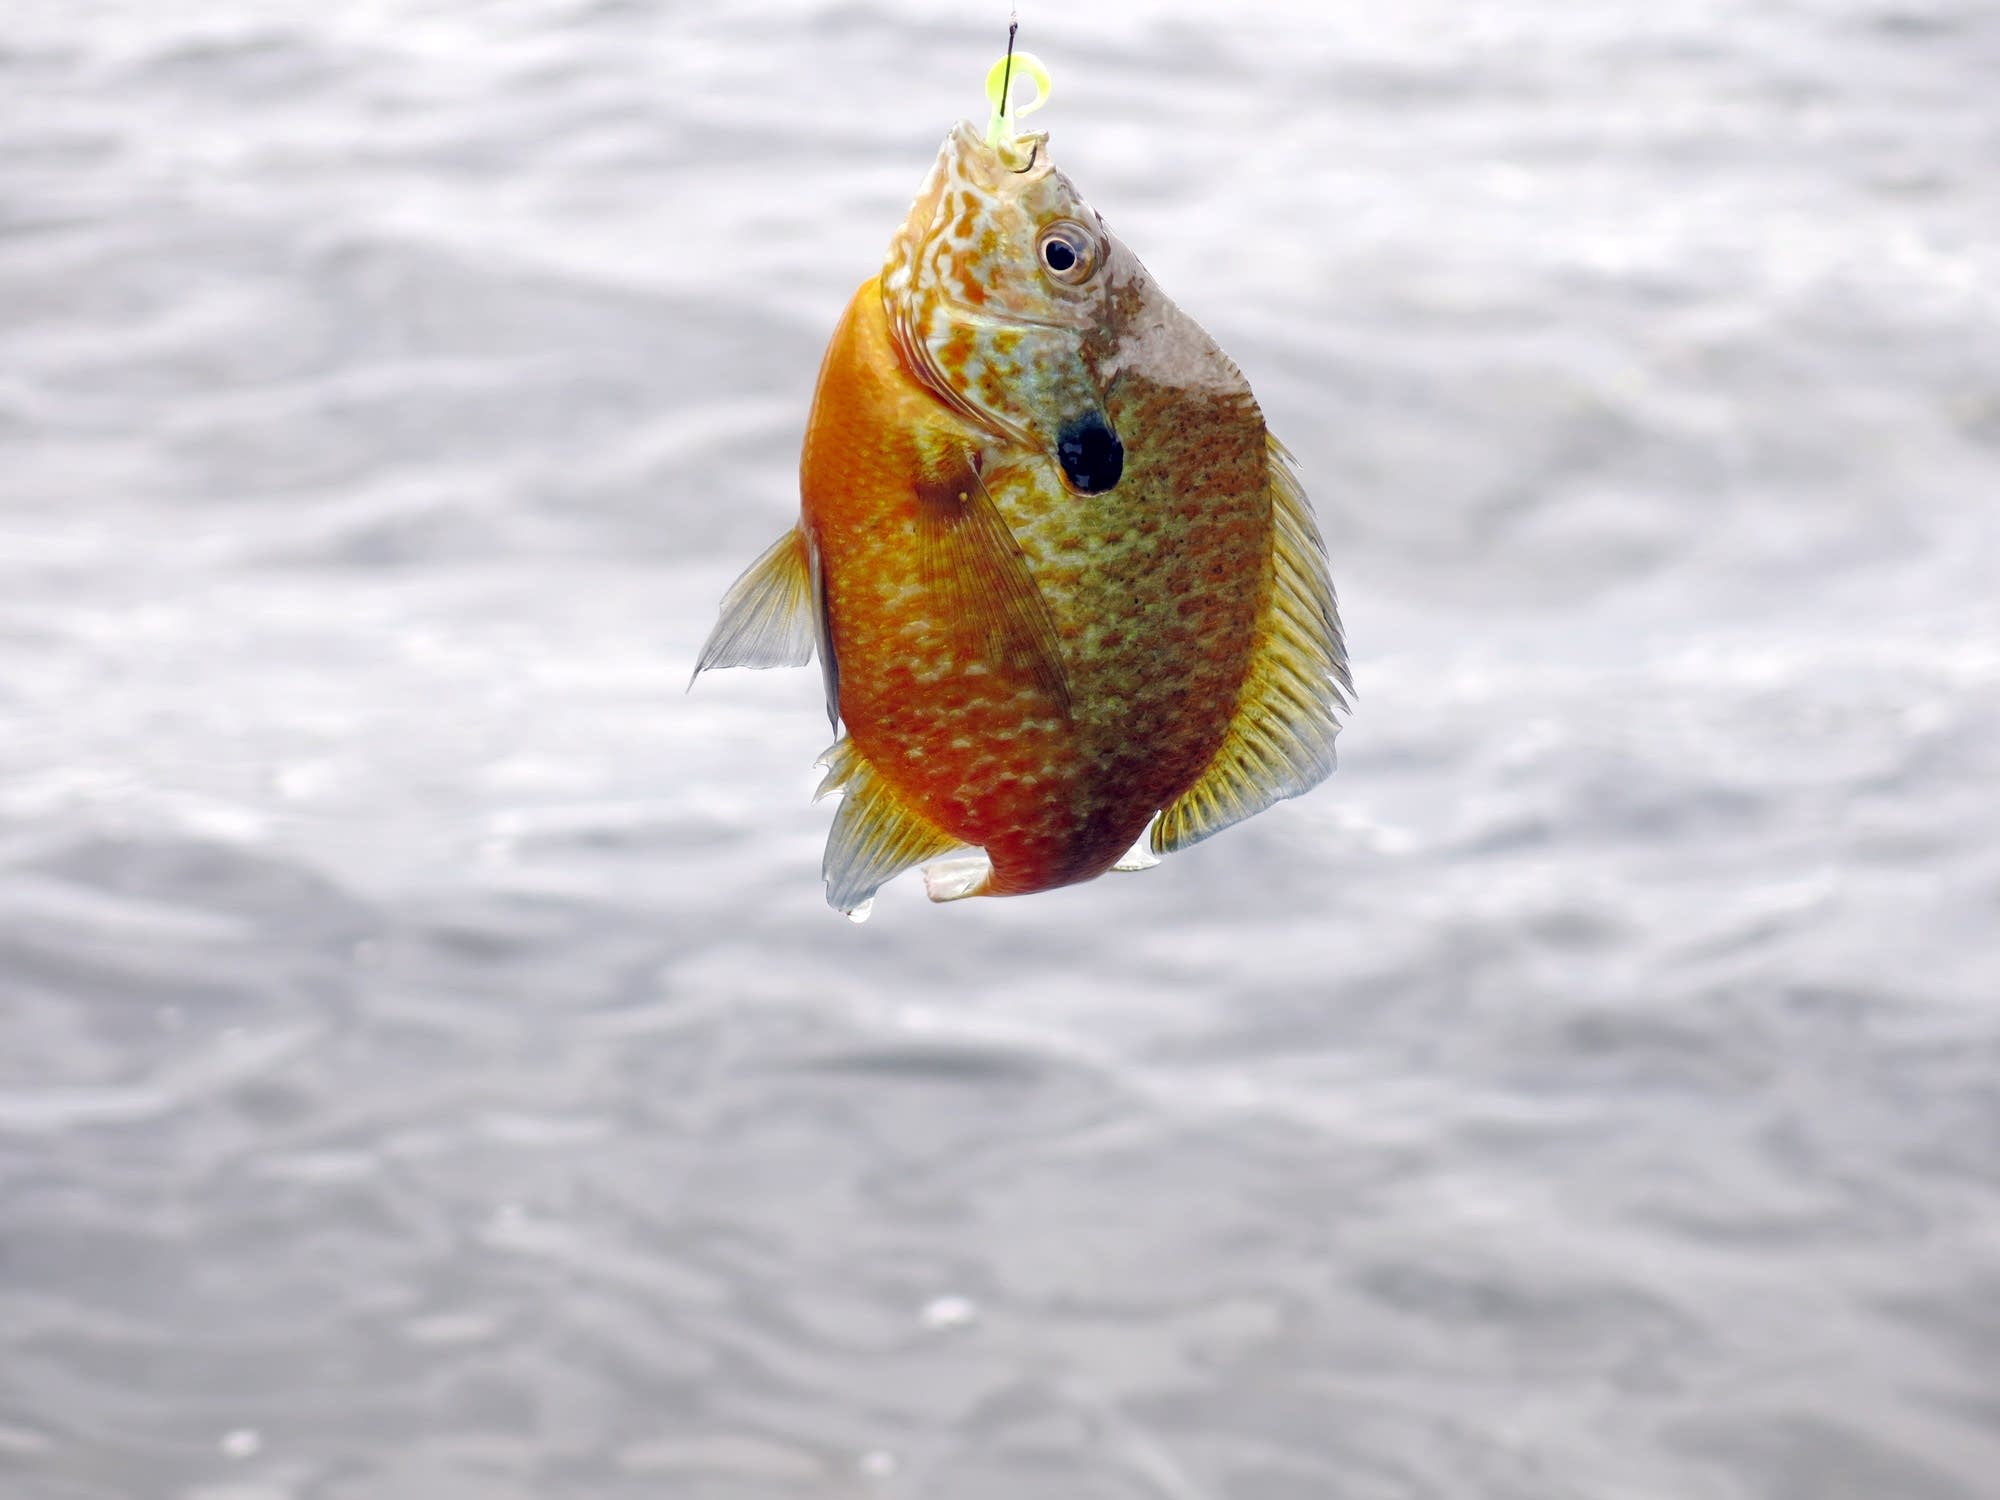
\includegraphics[width=.9\linewidth]{images/literature/colorfish}
        \caption{Original Image\cite{website:colorfish_image}}
    \end{subfigure}%
    \begin{subfigure}{.5\textwidth}
        \centering
        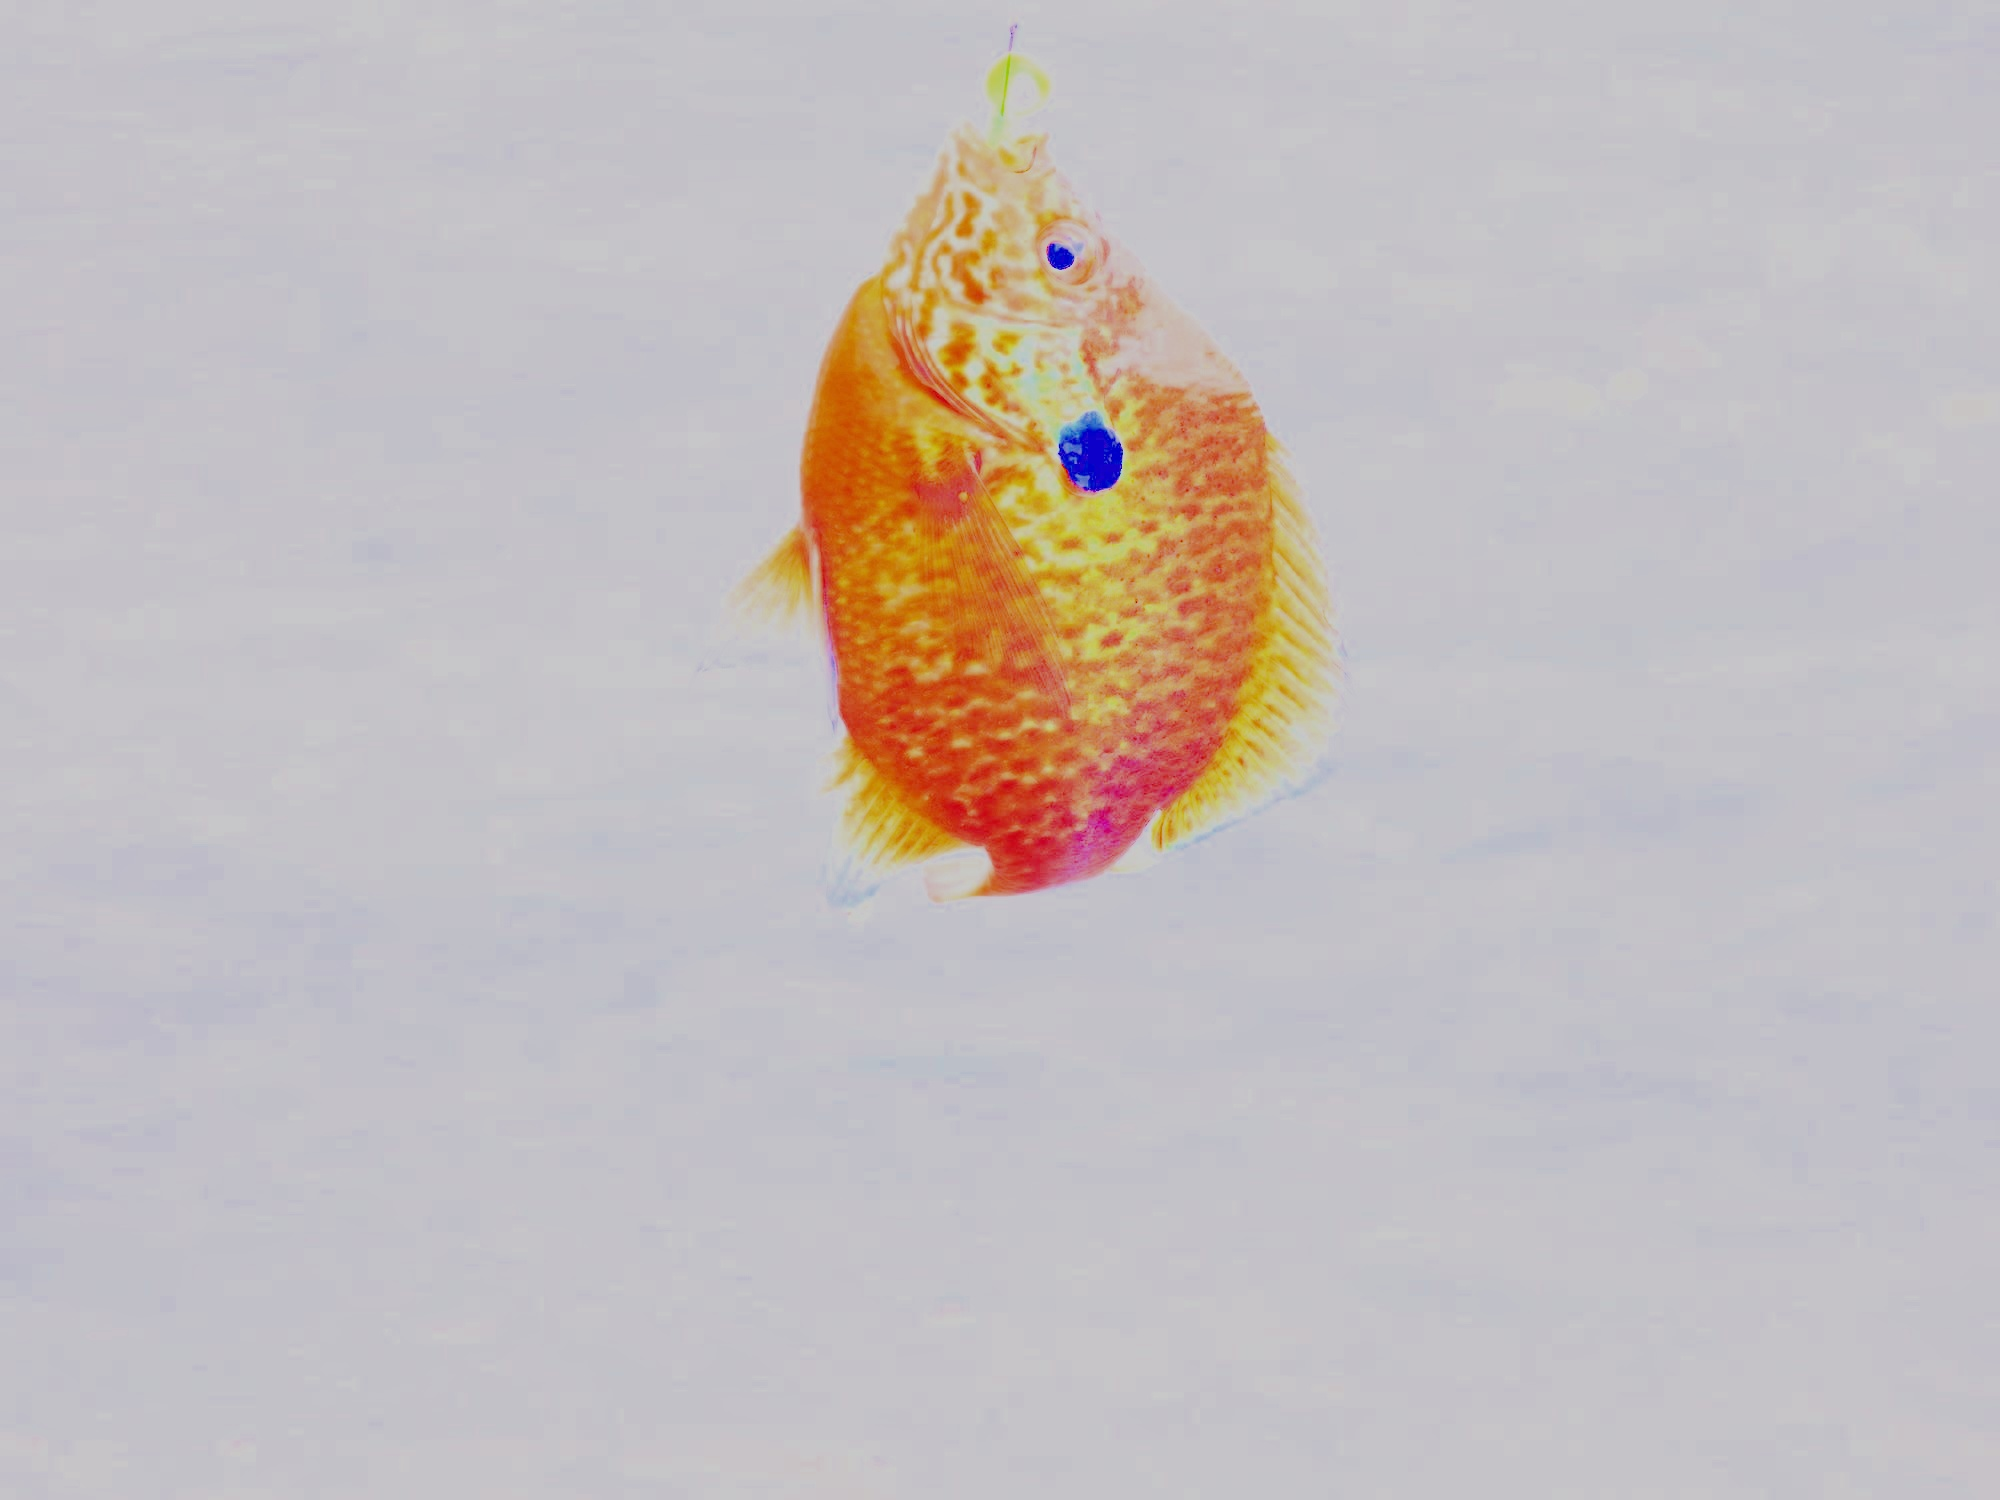
\includegraphics[width=.9\linewidth]{images/literature/shadow_removal}
        \caption{Shadow Removal}
    \end{subfigure}
    \caption{Example of shadow removal}
    \label{fig:shadow_removal}
\end{figure}

In figure \ref{fig:shadow_removal} it is shown that the colors of the fish is preserved, while all the shadows and blurry background in grey tones are evened out. In this example the value component is set to 200.

This type of simple shadow removal can be very useful, but for the image in figure \ref{fig:median_filter} the fish is not colorful enough for the technique to remove the shadows only.


%%%%%%%%%%%%%%%%%%%%%%%%%%%%%%%%%%%%%%%%%%%%%%%%%%%%%%%%%%%%%%%%%%%%%%

Depthmap Results:

\begin{figure}[H]
    \centering
    \begin{subfigure}{1\textwidth}
        \centering
        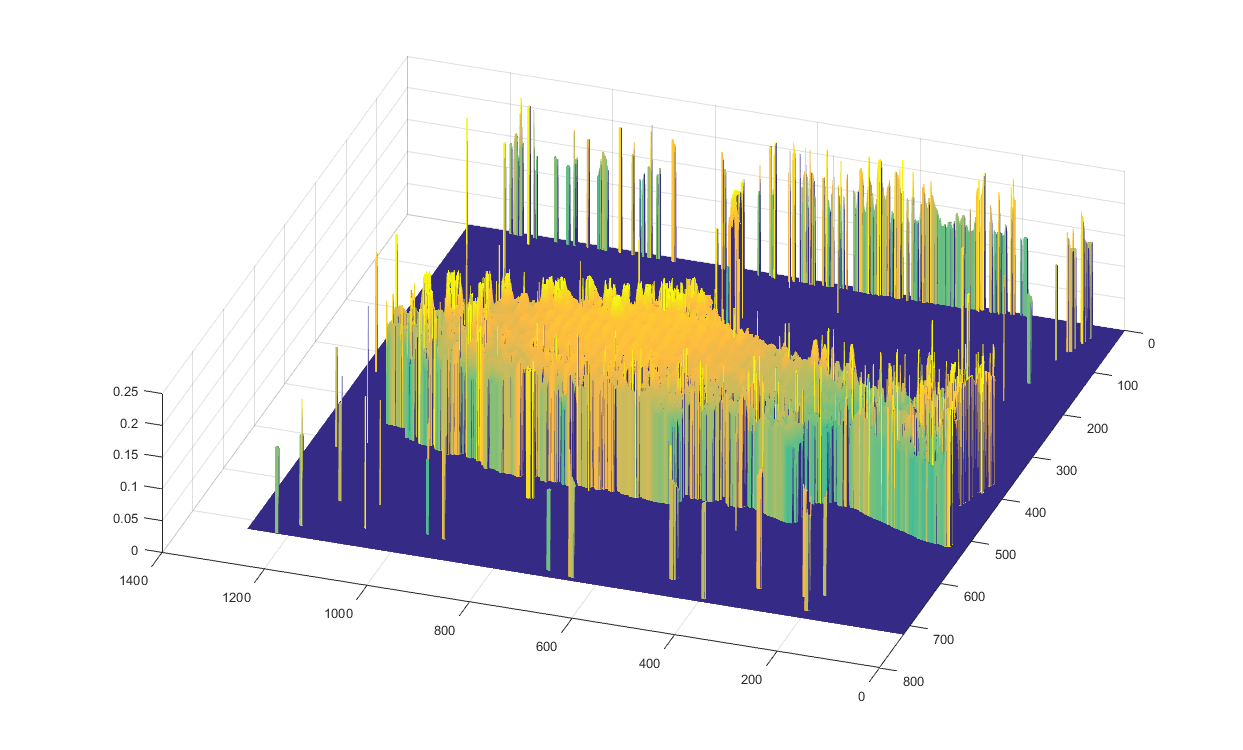
\includegraphics[width=.9\linewidth]{images/results/3D_plots/original_3D_63}
        \caption{Original depthmap} 
        \label{fig:3D_original_63}
    \end{subfigure}\hspace*{\fill}
    
    \medskip
    \begin{subfigure}{1\textwidth}
        \centering
        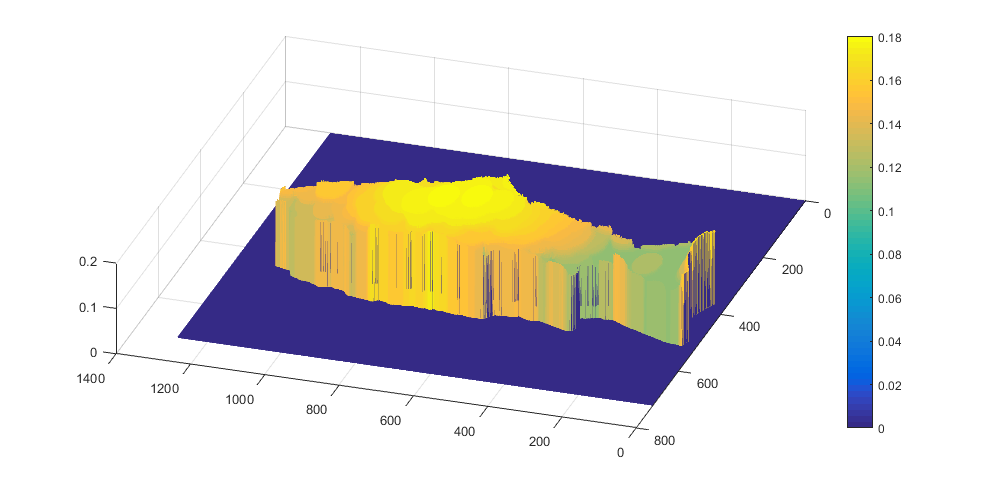
\includegraphics[width=.9\linewidth]{images/results/3D_plots/fixed_3D_63}
        \caption{Resulting depthmap} 
        \label{fig:3D_fixed_63}
    \end{subfigure}\hspace*{\fill}
    
    \medskip
    \begin{subfigure}{1\textwidth}
        \centering
        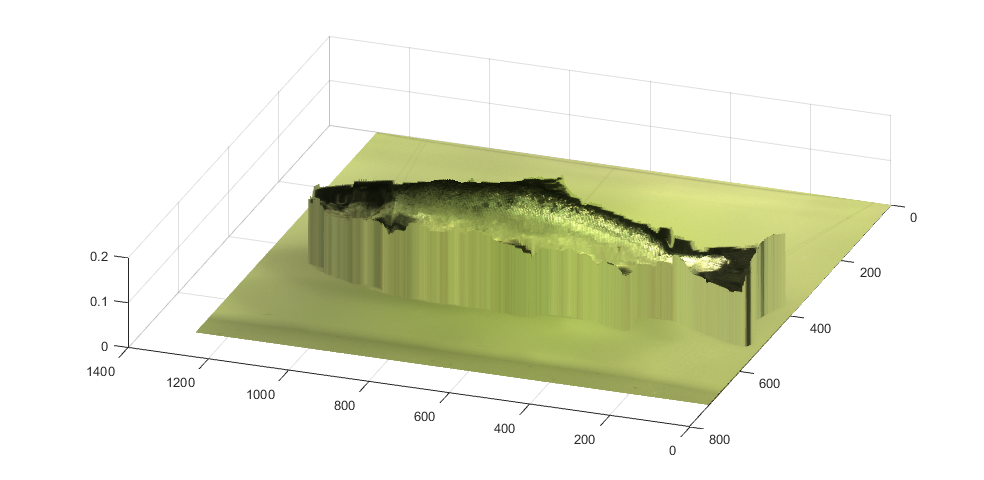
\includegraphics[width=.9\linewidth]{images/results/3D_plots/fixed_3D_fish_63}
        \caption{Resulting depthmap with image overlay} 
        \label{fig:3D_fixed_fish_63}
    \end{subfigure}\hspace*{\fill}
    \caption{3D plot of depthmap in MATLAB, number 563}
    \label{fig:3D_plot_63}
\end{figure}


\begin{figure}[H]
    \centering
    \begin{subfigure}{1\textwidth}
        \centering
        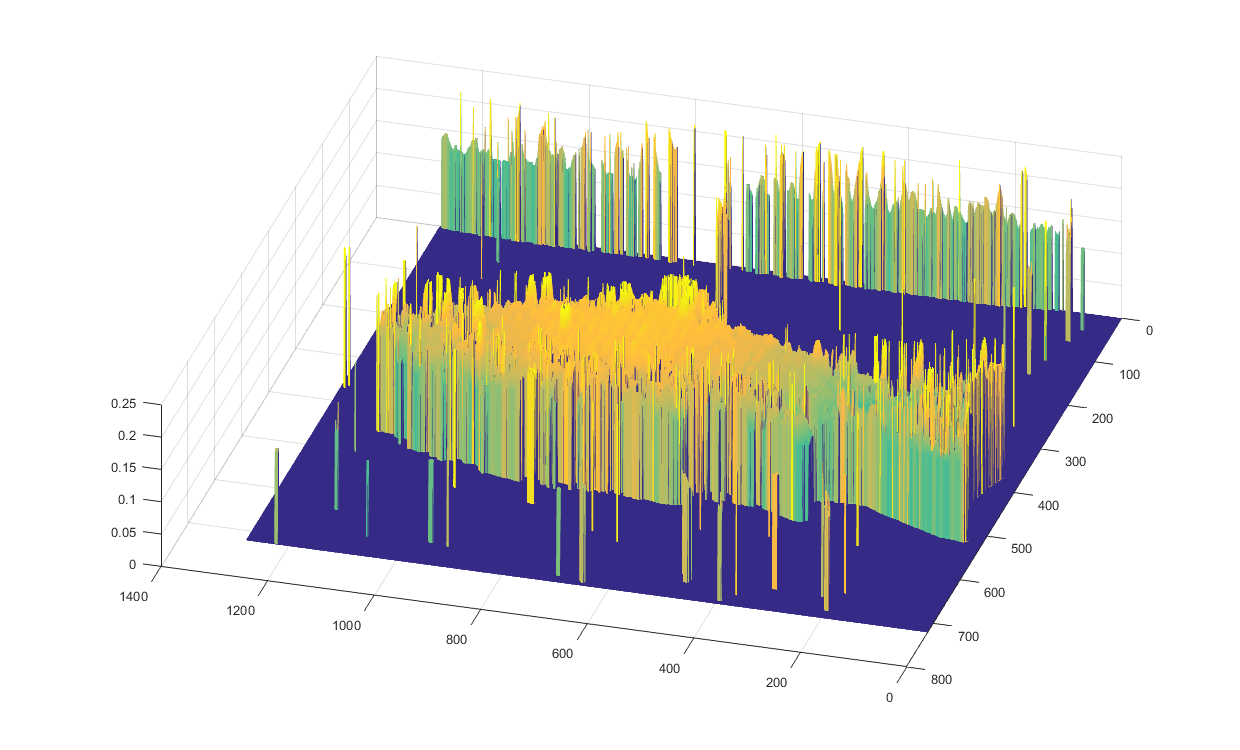
\includegraphics[width=.65\linewidth]{images/results/3D_plots/original_3D_87}
        \caption{Original depthmap} 
        \label{fig:3D_original_87}
    \end{subfigure}\hspace*{\fill}
    
    \medskip
    \begin{subfigure}{1\textwidth}
        \centering
        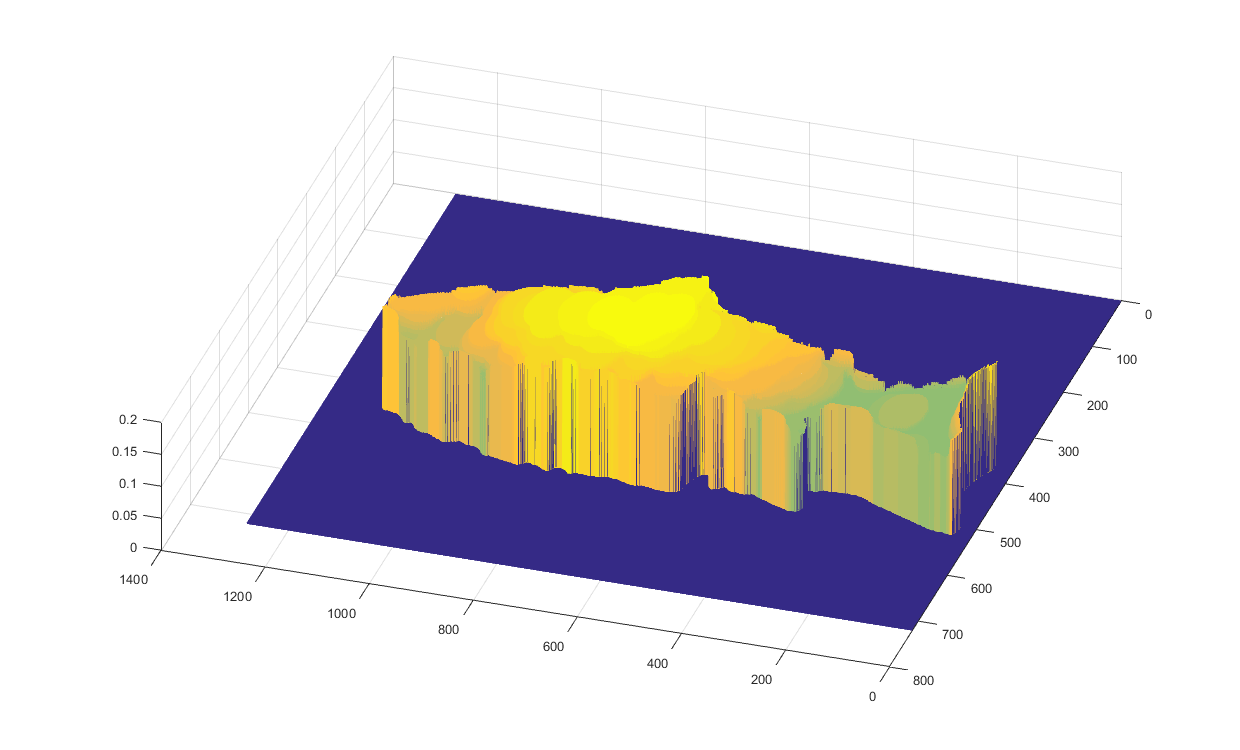
\includegraphics[width=.65\linewidth]{images/results/3D_plots/fixed_3D_87}
        \caption{Resulting depthmap} 
        \label{fig:3D_fixed_87}
    \end{subfigure}\hspace*{\fill}
    
    \medskip
    \begin{subfigure}{1\textwidth}
        \centering
        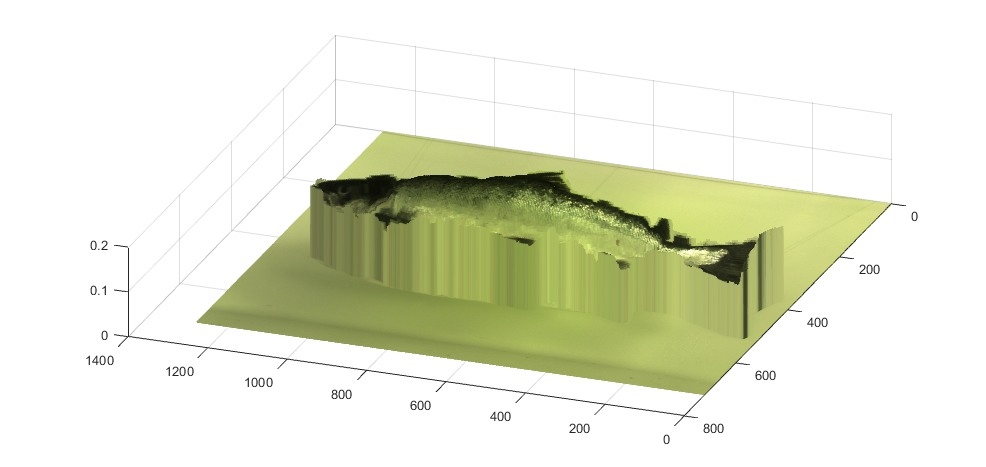
\includegraphics[width=.65\linewidth]{images/results/3D_plots/fixed_3D_fish_87}
        \caption{Resulting depthmap with image overlay} 
        \label{fig:3D_fixed_fish_87}
    \end{subfigure}\hspace*{\fill}
    \caption{3D plot of depthmap in MATLAB, number 587}
    \label{fig:3D_plot_87}
\end{figure}



%%%%%%%%%%%%%%%%%%%%%%%%%%%%%%%%%%%%%%%%%%%%%%%%%%%%%%%%%%%%%%


